\documentclass[tikz,border=2pt]{standalone}
\usepackage{amsmath}
\usetikzlibrary{arrows.meta}
\begin{document}
% M^B/M/1 sample path: batches of 3, 2, 1 jobs arrive at t=0, 2.2, 5 (blue up-jumps);
% services 1.0, 0.8, 1.2, 0.7, 0.9, 1.1 give departures at 1.0, 1.8, 3.0, 3.7, 4.6, 6.1 (red),
% each lowering L(t) by one; batch 2 waits from 2.2 to 3.0, so W^B = 0.8.
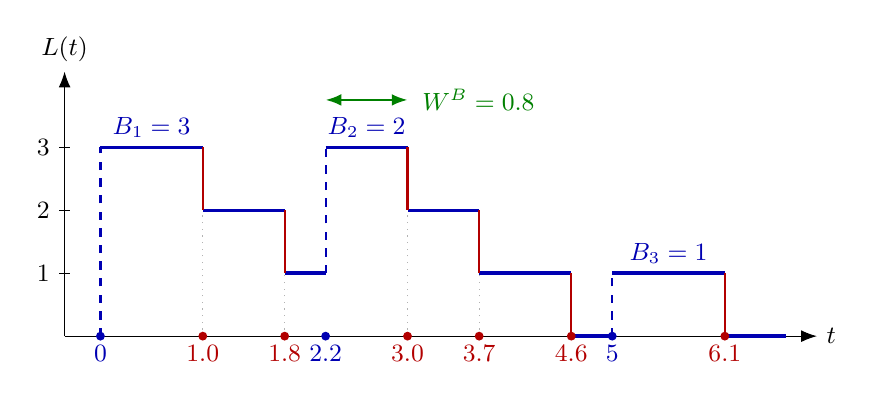
\begin{tikzpicture}[font=\small, >={Latex[length=2mm]}, x=1.3cm, y=0.8cm]
  \draw[->] (-0.35,0) -- (7.0,0) node[right] {$t$};
  \draw[->] (-0.35,0) -- (-0.35,4.2) node[above] {$L(t)$};
  \foreach \y in {1,2,3} \draw (-0.4,\y) -- (-0.3,\y) node[pos=0, left] {$\y$};
  % sample path
  \draw[blue!70!black, very thick]
    (0,3) -- (1.0,3) (1.0,2) -- (1.8,2) (1.8,1) -- (2.2,1) (2.2,3) -- (3.0,3)
    (3.0,2) -- (3.7,2) (3.7,1) -- (4.6,1) (4.6,0) -- (5.0,0) (5.0,1) -- (6.1,1) (6.1,0) -- (6.7,0);
  % batch jumps
  \draw[blue!70!black, thick, dashed] (0,0) -- (0,3);
  \fill[blue!70!black] (0,0) circle (1.6pt);
  \fill[blue!70!black] (2.2,0) circle (1.6pt);
  \fill[blue!70!black] (5.0,0) circle (1.6pt);
  \draw[blue!70!black, thick, dashed] (2.2,1) -- (2.2,3);
  \draw[blue!70!black, thick, dashed] (5.0,0) -- (5.0,1);
  \node[blue!70!black, anchor=south] at (0.5,3) {$B_1=3$};
  \node[blue!70!black, anchor=south] at (2.6,3) {$B_2=2$};
  \node[blue!70!black, anchor=south] at (5.55,1) {$B_3=1$};
  % departures
  \foreach \d/\hi in {1.0/3,1.8/2,3.0/3,3.7/2,4.6/1,6.1/1} {
    \draw[red!70!black, thick] (\d,\hi) -- (\d,\hi-1);
    \draw[gray!60, thin, dotted] (\d,0) -- (\d,\hi-1);
    \fill[red!70!black] (\d,0) circle (1.6pt);
  }
  \foreach \d in {1.0,1.8,3.0,3.7,4.6,6.1} \node[red!70!black, below] at (\d,0) {$\d$};
  \foreach \a in {2.2,5} \node[blue!70!black, below] at (\a,0) {$\a$};
  \node[blue!70!black, below] at (0,0) {$0$};
  % batch waiting time of batch 2
  \draw[<->, green!50!black, thick] (2.2,3.75) -- (3.0,3.75);
  \node[green!50!black, anchor=west] at (3.05,3.75) {$W^B=0.8$};
\end{tikzpicture}
\end{document}
